\section*{Abstract}
Replication studies are increasingly conducted in order to confirm original
findings. However, there is no established standard how to assess replication
success and in practice many different approaches are used. The purpose of this
paper is to refine and extend a recently proposed reverse-Bayes approach for the
analysis of replication studies. We show how this method is directly related to
the relative effect size, the ratio of the replication to the original effect
estimate. This perspective leads to a new proposal to recalibrate the assessment
of replication success, the golden level. The recalibration ensures that for
borderline significant original studies replication success can only be achieved
if the replication effect estimate is larger than the original one. Conditional
power for replication success can then take any desired value if the original
study is significant and the replication sample size is large enough. Compared
to the standard approach to require statistical significance of both the
original and replication study, replication success at the golden level offers
uniform gains in project power and controls the Type I error rate if the
replication sample size is not smaller than the original one. An application to
data from four large replication projects shows that the new approach leads to
more appropriate inferences, as it penalizes shrinkage of the replication
estimate compared to the original one, while ensuring that both effect estimates
are sufficiently convincing on their own.

\textbf{Key words}: Power, replication studies, sceptical $p$-value, shrinkage,
two-trials rule, type I error rate

\section{Introduction}
Replication studies are conducted in order to investigate whether an original
finding can be confirmed in an independent study. Although replication has long
been a central part of the scientific method in many fields, the so-called
replication crisis \citep{Ioannidis2005, Begley2015} has led to increased
interest in replication over the last decade. These developments eventually
culminated in large-scale replication projects that were conducted in various
fields \citep{Errington2014, Klein2014, Opensc2015, Ebersole2016, Camerer2016,
  Camerer2018, Cova2018, Klein2018}.

Declaring a replication as successful is, however, not a straightforward task,
and currently used approaches include statistical significance of both the
original and replication study, compatibility of their effect estimates, and
meta-analysis of the effect estimates. Many of the replication projects listed
above also report the relative effect size, the ratio of the replication to the
original effect estimate. For example, in \citet{Camerer2018} the replication
effect estimates were only half as large as the original ones on average and
even smaller in \citet{Opensc2015}. This gives clear evidence of a systematic
bias of the original studies and strongly suggests that the original and
replication study should not be treated as exchangeable. However, all the
approaches mentioned above will give the same results if the order of studies
would be reversed.

In order to address this problem, a new method has recently been proposed in
\citet{Held2020}. The approach combines the analysis of credibility
\citep{Matthews2001a,Matthews2001b} with a prior-data conflict assessment
\citep{Box1980}. Replication success is declared if the replication study is in
conflict with a sceptical prior that would make the original study
non-significant. This approach penalizes small relative effect sizes as we will
see in more detail in the following.



To introduce some notation, let $z_o = \hat \theta_o/\sigma_o$ and
$z_r = \hat \theta_r/\sigma_r$ denote the $z$-statistic of the original and
replication study, respectively. Here $\hat \theta_o$ and $\hat \theta_r$ are
the corresponding effect estimates (assumed to be normally distributed) of the
unknown effect $\theta$ with standard errors $\sigma_o$ and $\sigma_r$,
respectively. The corresponding one-sided $p$-values are denoted by
$p_o=1-\Phi(z_o)$ and $p_r=1-\Phi(z_r)$, respectively, where $\Phi(\cdot)$
denotes the standard normal cumulative distribution function. Let
$c = \sigma_o^2/\sigma_r^2$ denote the variance ratio of the squared standard
errors of the original and replication effect estimates. The squared standard
errors are usually inversely proportional to the sample size of each study, \ie{}
$\sigma_o^2 = \kappa^2/n_o$ and $\sigma_r^2 = \kappa^2/n_r$ for some unit
variance $\kappa^2$. The variance ratio $c$ can then be identified as the
relative sample size $c=n_r/n_o$. The relative effect size
\begin{equation}\label{eq1:d}
  d = \frac{\hat \theta_r}{\hat \theta_o} = \frac{1}{\sqrt{c}} \frac{z_r}{z_o}
\end{equation}
quantifies the size of the replication effect estimate $\hat \theta_r$ relative
to the original effect estimate $\hat \theta_o$. The corresponding shrinkage of
the replication effect estimate will be denoted as $s=1-d$.

Suppose the original study achieved statistical significance at one-sided level
$\alpha$, so $p_o \leq \alpha$. The standard approach to assess replication
success is based on significance of the replication effect estimate at the same
level $\alpha$, \ie{} the replication is considered successful if also
$p_r \leq \alpha$. This approach is known in drug development as the two-trials
rule \citep{Senn2008}, usually conducted at $\alpha=0.025$. Let
$z_\alpha = \Phi^{-1}(1-{\alpha})>0$ denote the $z$-value corresponding to the
level $\alpha$, then significance of the replication study is achieved if
$z_r \geq z_\alpha$, which is equivalent to the condition
\begin{equation}\label{eq1:dSig}
   d \geq \frac{z_\alpha}{z_o  \, \sqrt{c}}
\end{equation}
on the relative effect size \eqref{eq1:d}. The right hand-side goes to zero for
increasing $c$, so if the relative sample size $c$ is large enough, significance
of the replication study can be achieved with any arbitrarily small (but
positive) relative effect size $d$. However, declaring replication success when
there is substantial shrinkage is contrary to common sense, as the replication
effect estimate may not reflect an effect size of the same practical relevance
as the original one, despite its statistical significance.

In this paper we first review the \citet{Held2020} approach for the assessment
of replication success, followed by showing how it relates to the relative
effect size (Section \ref{sec1:res}). This perspective is used in Section
\ref{sec1:goldenthresh} and \ref{sec1:recalib} to propose a recalibration of the
method, the \textit{golden level}, which leads to a more appropriate criterion
for replication success compared to the two-trials rule (Section \ref{sec1:2TR}).
In Section \ref{sec1:ER} we study power and Type I error rates of the proposed
method and compare it to the two-trials rule. The recalibrated method ensures
that conditional power can take any desired value if the original study has been
significant and the replication sample size is large enough (Section
\ref{sec1:powerrep}), controls the overall Type I error if the replication sample
size is not smaller than the original one (Section \ref{sec1:T1E}), and offers
uniform gains in project power compared to the two-trials rule (Section
\ref{sec1:PP}). Section \ref{sec1:application} describes an application to data
from four replication projects and Section \ref{sec1:discussion} closes with some
discussion.

\section{Replication success}\label{sec1:RS}

\begin{center}
\begin{figure}[!h]
\begin{center}
\begin{knitrout}
\definecolor{shadecolor}{rgb}{0.969, 0.969, 0.969}\color{fgcolor}

{\centering 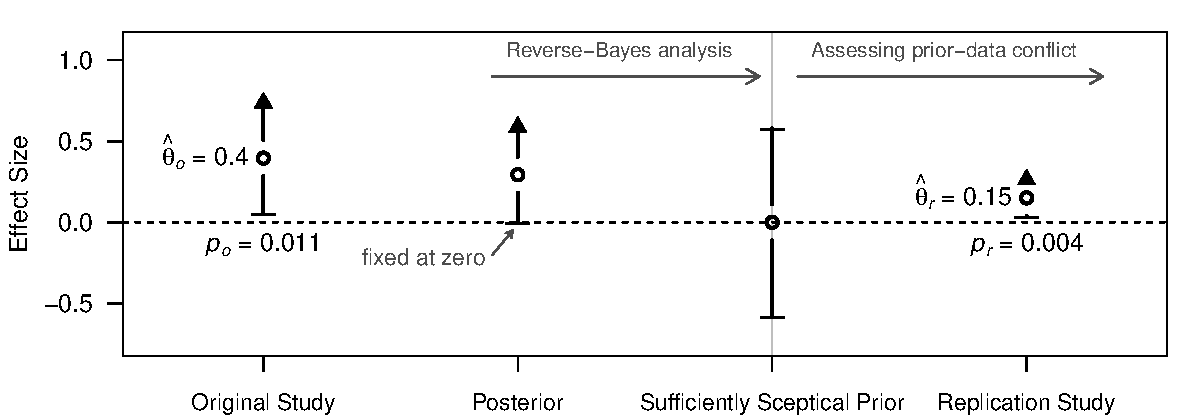
\includegraphics[width=\maxwidth]{images/paper1/fig1-1}

}

\end{knitrout}
\caption{Example of the assessment of replication success. The original study
  from \citet{Pyc2010} has effect estimate $\hat \theta_o= 0.4$ on Fisher's $z$
  scale (95\% CI from $0.05$ to $0.74$) and one-sided $p$-value $p_o = 0.011$.
  The left part of the figure illustrates the reverse-Bayes derivation of the
  sufficiently sceptical prior based on the original study result and the
  posterior with lower credible limit fixed at zero. The comparison of the
  sufficiently sceptical prior with the replication study result
  ($\hat \theta_r = 0.15$, 95\% CI from 0.04 to 0.26, $p_r = 0.004$) in the
  right part of the figure is used to assess potential prior-data conflict.}
  \label{fig1:fig1}
\end{center}
\end{figure}
\end{center}



Hereinafter we focus on the one-sided assessment of replication success to
ensure that replication success can only occur if the original and replication
effect estimates go in the same direction. Figure \ref{fig1:fig1} illustrates the
\citet{Held2020} approach based on a replication study from the \textit{Social
  Sciences Replication Project} \citep{Camerer2018}: the significant original
finding by \citet{Pyc2010} at one-sided level $\alpha=0.025$ is challenged with
a sceptical prior, sufficiently concentrated around zero to make the original
study result no longer convincing \citep{Matthews2001a,Matthews2001b}.
Replication success is then defined as conflict between the sceptical prior and
the result from the replication study in order to disprove the sceptic. Conflict
is quantified by a prior-predictive tail probability $p_{\mbox{\scriptsize
    Box}}$ \citep{Box1980} where a small value $p_{\mbox{\scriptsize
    Box}} \leq \alpha$ defines replication success. In Figure \ref{fig1:fig1} the
original finding is only borderline significant, so the sufficiently sceptical
prior is fairly wide. Furthermore, there is substantial shrinkage
($d = 0.15/0.4 = 0.38$) of the replication effect estimate and therefore hardly
any conflict with the sufficiently sceptical prior (one-sided
$p_{\mbox{\scriptsize Box}}=0.31$). We are thus not able to declare replication
success at level $2.5$\%.

The actual value of $p_{\mbox{\scriptsize Box}}$ is difficult to interpret as it
depends on the level $\alpha$ and does not even exist if the original $p$-value
$p_o$ exceeds $\alpha$. However, \citet{Held2020} showed that if both
$\sign(z_o)=\sign(z_r)$ and
\begin{equation}\label{eq1:extrinsic.p}
\left({z_o^2}/{z_{{\alpha_S}}^2}-1 \right) \left({z_r^2}/{z_{{\alpha_S}}^2}
- 1 \right) \geq c
\end{equation}
hold, replication success at level ${\alpha_S}$ is achieved, where
$z_{{\alpha_S}} = \Phi^{-1}(1-{\alpha_S})$. The requirement
\eqref{eq1:extrinsic.p} can be assessed for any value of
${{\alpha_S}} > \max\{p_o, p_r\}$ and of particular interest is the smallest
possible value of $\alpha_S$ where \eqref{eq1:extrinsic.p} holds, the so-called
\textit{sceptical $p$-value} $p_S$. We are thus interested in the value $z_S^2$
that fulfills
\begin{equation}\label{eq1:extrinsic.p2}
\left({z_o^2}/{z_{S}^2}-1 \right) \left({z_r^2}/{z_{S}^2}
- 1 \right) = c.
\end{equation}
There is a unique solution of \eqref{eq1:extrinsic.p2} which defines the
one-sided {sceptical $p$-value} $p_S= 1-\Phi\left({z_S}\right)$ where
$z_{S} \coloneqq + \surd z_{S}^2$, provided $\sign(z_o)=\sign(z_r)$ holds.
Replication success at level $\alpha_S$ is then achieved if $p_S \leq \alpha_S$.
In the introductory example based on the original study by \citet{Pyc2010}, the
sceptical $p$-value turns out to be $p_S=0.11$.

The sceptical $p$-value has a number of interesting properties, see
\citet[Section 3.1]{Held2020} for details. In particular,
$p_S > \max\{p_o, p_r\}$ always holds with $p_S \downarrow \max\{p_o, p_r\}$ for
$c \downarrow 0$. Furthermore, if the $p$-values $p_o$ and $p_r$ are fixed, the
sceptical $p$-value $p_S$ increases with decreasing relative effect size $d$.
The first property ensures that both the original and the replication study have
to be sufficiently convincing on their own to achieve replication success. The
second property guarantees that shrinkage of the replication effect estimate is
penalized.

The level for replication success $\alpha_S$ has to be distinguished from the
significance level $\alpha$ associated with the ordinary $p$-value.
\citet{Held2020} has used the \textit{nominal level} for replication success
($\alpha_S=\alpha$) for convenience, but in the following we will propose a
recalibration of the procedure along with a new value for $\alpha_S$, the
\textit{golden level} (Section~\ref{sec1:goldenthresh}). The derivation is based
on a property of the required relative effect size for replication success, if
the relative sample size is very large (Section~\ref{sec1:res}). In a nutshell,
the golden level ensures that for original studies which were only borderline
significant ($p_o=\alpha$), replication success is only possible if the
replication
effect estimate is larger than the original one ($d > 1$).\\


\subsection{Relative effect size}\label{sec1:res}
Without loss of generality we now assume that $\hat \theta_o > 0$ and that
$p_o < {\alpha_S}$ has been observed in the original study, otherwise it would
be impossible to achieve replication success at level $\alpha_S$ because $p_S$
is always larger than $p_o$. The condition \eqref{eq1:extrinsic.p} for
replication success can then be re-written as
\begin{equation}\label{eq1:eq.z}
  z_r \geq   z_{{\alpha_S}} \sqrt{1+c/(K-1)} \eqqcolon  \zrmin,
\end{equation}
where $K=z_o^2/z_{{\alpha_S}}^2>1$. The right hand-side of \eqref{eq1:eq.z} is
the minimum replication $z$-value $\zrmin$ required to achieve replication
success. Note that $\zrmin$ increases with increasing $c$, so increasing the
replication sample size leads to a more stringent success requirement $z_r$ and
the corresponding replication $p$-value $p_r$.

Equation \eqref{eq1:eq.z} can be further transformed to a
condition on the relative effect size \eqref{eq1:d}:
\begin{equation}\label{eq1:res}
  d \geq  \frac{\sqrt{1+c/(K-1)}}{ \sqrt{c K}} \eqqcolon \dmin .
\end{equation}
To achieve replication success, the relative effect size must be at least as
large as the right hand-side of \eqref{eq1:res}, the minimum relative effect size
$\dmin$, a function of $K$ and the relative sample size $c$. If the relative
sample size becomes very large, \ie{} $c \rightarrow \infty$, we have
$\dmin \downarrow \dinfty$ where
\begin{equation}\label{eq1:smallestpossible}
  \dinfty = 1/\sqrt{K (K-1)}
\end{equation}
is the \textit{limiting relative effect size}. This shows that the minimum
relative effect size $\dmin$ in \eqref{eq1:res} does not go to zero for
increasing $c$, so replication success cannot be achieved if the relative effect
size $d$ is smaller or equal to $\dinfty$, no matter how large the replication
study is. In contrast, the corresponding criterion \eqref{eq1:dSig} of the
two-trials rule can be achieved for any positive relative effect size,
regardless of how small, provided the replication sample size is sufficiently
large.


\subsection{The golden level}\label{sec1:goldenthresh}
Significance of both the original and the replication study at level $\alpha$ is
a necessary but not sufficient requirement for replication success at the
nominal level ($\alpha_S = \alpha$). The nominal level may therefore be too
stringent. It is more reasonable to calibrate the procedure in such a way that
to establish replication success, original and replication study do not both
necessarily need to be significant at level $\alpha$, provided that the
replication effect estimate does not shrink compared to the original one. We
therefore choose a level $\alpha_S$ such that a borderline significant original
study ($p_o = \alpha$) cannot lead to replication success if there is shrinkage
$s > 0$ of the replication effect estimate. Mathematically, this translates to
setting $\dinfty = 1$ and $K = z_\alpha^2/z_{\alpha_S}^2$
in~\eqref{eq1:smallestpossible} and leads to the quadratic equation $K(K-1) = 1$
with solution $K = \varphi$ where $\varphi = (\sqrt{5}+1)/2 \approx 1.62$ is
known as the golden ratio. Solving for $z_{\alpha_S}$ gives
$z_{\alpha_S} = z_\alpha / \sqrt{\varphi}$ and the corresponding \textit{golden
  level}
\begin{eqnarray}\label{eq1:golden}
\alpha_S & = & 1 -  \Phi(z_\alpha / \sqrt{\varphi} )
\end{eqnarray}
for replication success. This is our recommended default choice to assess
replication success and we will study its properties in the following in more
detail. For $z_\alpha = 1.96$ (one-sided $\alpha = 0.025$), the golden level is
$\alpha_S =0.062$. In the introductory example shown in Figure \ref{fig1:fig1},
the sceptical $p$-value is $p_S=0.11 > 0.062$, so the replication of the
\citet{Pyc2010} study was not successful.




The golden level \eqref{eq1:golden} is derived from~\eqref{eq1:smallestpossible}
with $\dinfty = 1$. However, we may also use a different value for the limiting
relative effect size $\dinfty$, say $\dinfty=0.8$. Then replication success is
only possible for a borderline significant result ($p_o = \alpha$) if there is
less than $1-\dinfty$ (20\% for $\dinfty=0.8$) shrinkage of the replication
effect estimate. This approach is equivalent to a limiting relative effect size
of 1 if the original $p$-value $p_o$ is equal to a different level $\alpha'$,
which can be derived as follows: First, solving \eqref{eq1:smallestpossible} for
$\dinfty > 0$ gives
$K = z_\alpha^2/z_{\alpha_S}^2 = 1/2+\sqrt{1/4 + 1/\dinfty^2}$. The new level
$\alpha'$ fulfills $\varphi=z_{\alpha'}^2/z_{\alpha_S}^2$, so
$z_\alpha^2/K=z_{\alpha'}^2/\varphi$ and therefore
\begin{equation}\label{eq1:alphaPrime}
\alpha' = 1-\Phi\left(z_{\alpha} \, \sqrt{\varphi / K} \right).
\end{equation}
For example, for $\alpha = 0.025$ and $\dinfty = 0.8$ we obtain $\alpha'=0.033$.


\subsection{Recalibration of the sceptical \textit{p}-value}\label{sec1:recalib}

The condition $p_S \leq \alpha_S$ for replication success at the golden level is
equivalent to $z_S \geq z_\alpha / \sqrt{\varphi}$, \ie{}
$z_S \sqrt{\varphi} \geq z_\alpha$. In practice it may be preferable to
recalibrate the sceptical $p$-value $p_{S} = 1 - \Phi(z_S)$ to
$ \tilde{p}_S = 1 - \Phi(z_S \sqrt{\varphi})$, which then needs to be compared
to $\alpha$ (rather than $\alpha_S$) to assess replication success and can thus
be interpreted on the same scale as an ordinary $p$-value. For example, the
recalibrated sceptical $p$-value for the replication of \citet{Pyc2010} turns
out to be $\tilde{p}_S=0.061$ and does not lead to replication success at any
level $\alpha<0.061$, including the standard $0.025$ level.


\subsection{Comparison with the two-trials rule}\label{sec1:2TR}
A useful benchmark for comparison is the two-trials rule in drug development
\citep[Section 9.4]{Kay2015}, which requires ``at least two adequate and
well-controlled studies, each convincing on its own, to establish
effectiveness'' \citep[p.~3]{FDA1998}. This is usually achieved by independently
replicating the result of a first study in a second study, both significant at
one-sided level $\alpha=0.025$. {It is worth noting that in practice the two
  trials are often run in parallel} {\citep{Senn2008}}{, so do not exactly
  resemble the replication setting.}



The main difference between the replication success and the two-trials
rule approach concerns how shrinkage of the replication effect
estimate is handled. Figure~\ref{fig1:fig2} illustrates that
shrinkage is penalized in the assessment of replication success, \ie{}
the original $p$-value needs to be quite small to achieve replication
success for a relative effect size $d<1$. In contrast, significance of
the replication study can be achieved even if there is substantial
shrinkage, provided the replication sample size is large enough.


\begin{figure}[!h]
\centering
\begin{knitrout}
\definecolor{shadecolor}{rgb}{0.969, 0.969, 0.969}\color{fgcolor}

{\centering 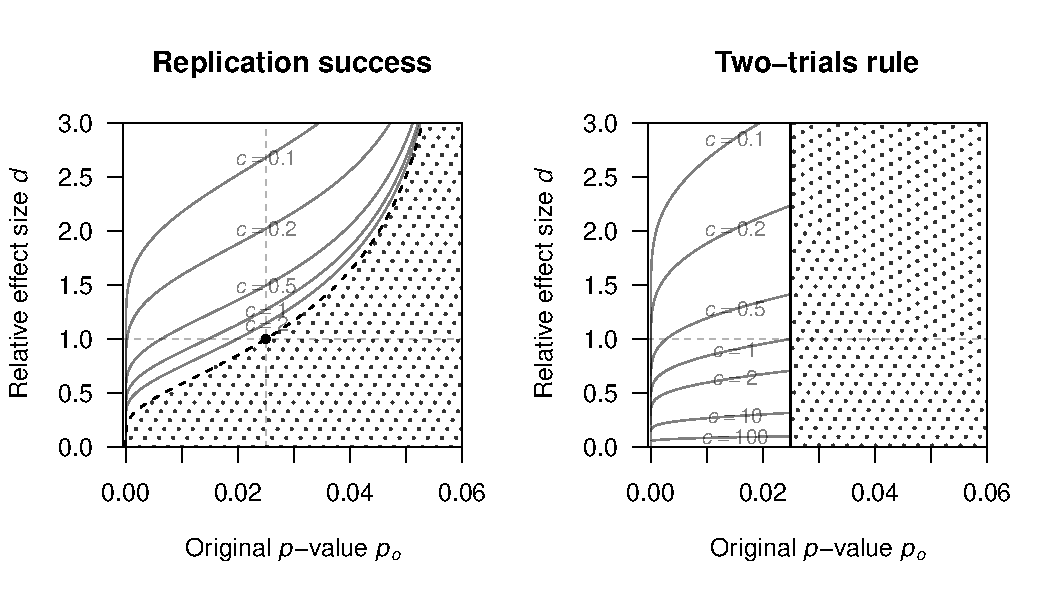
\includegraphics[width=\maxwidth]{images/paper1/fig2-1}

}


\end{knitrout}
\caption{Comparison of replication success at the golden level
  ($p_S \leq \alpha_S = 0.062$) and the two-trials rule ($p_o \leq 0.025$ and
  $p_r \leq 0.025$). The dotted areas indicate that success is impossible for
  original $p$-value $p_o$ and relative effect size $d$. In the white areas
  success is possible and depends on the relative sample size $c$ as indicated
  by the grey lines. The dashed black line in the left plot indicates the
  limiting relative effect size $\dinfty$. }
\label{fig1:fig2}
\end{figure}



It is interesting to directly compare the two-trials rule and replication
success at the golden level in terms of the required relative effect size $d$ to
fulfill the criteria \eqref{eq1:dSig} and \eqref{eq1:res}, respectively, see
Figure~\ref{fig1:fig2}. If the original $p$-value is not significant at level
$\alpha$, only replication success can be achieved, but will require a
replication effect estimate larger than the original one.

For example, four studies with one-sided $p_o \in (0.025, 0.03)$ have been
included in the \textit{Reproducibility Project: Psychology} \citep{Opensc2015}
and one of them achieves replication success (see Section \ref{sec1:application}
for details). By definition, such non-significant original findings can never
fulfill the two-trials rule.

If the original $p$-value is smaller than $\alpha$, then the situation depends
on the relative sample size $c$. For example, when the replication sample size
is chosen to be the same as in the original study ($c=1$) and $\alpha=0.025$,
original studies with a $p$-value larger than $0.006$ will require a smaller
relative effect size $d$ with the two-trials rule, while $p$-values smaller than
$0.006$ will require a smaller relative effect size $d$ with the replication
success method. This illustrates that the latter method is less stringent than
the two-trials rule if the original study is already sufficiently convincing.

\section{Power and Type I Error Rate}\label{sec1:ER}
Although Bayesian methods do not rely on the frequentist paradigm of repeated
testing, it is still useful to investigate their frequentist operating
characteristics \citep{Dawid1982, Rubin1984, Grieve2016} and this also holds for
the proposed reverse-Bayes assessment of replication success. We first condition
on the results from the original study and compare the power to achieve
replication success with the two-trials rule in Section \ref{sec1:powerrep}. We
then assume that none of the two studies have been conducted and investigate the
overall Type I error rate (Section \ref{sec1:T1E}) and the project power (Section
\ref{sec1:PP}) \citep{Maca2002} over both studies in combination for fixed
relative sample size $c$.

\subsection{Conditional power}\label{sec1:powerrep}


\begin{figure}[!ht]
\begin{center}
\begin{knitrout}
\definecolor{shadecolor}{rgb}{0.969, 0.969, 0.969}\color{fgcolor}

{\centering 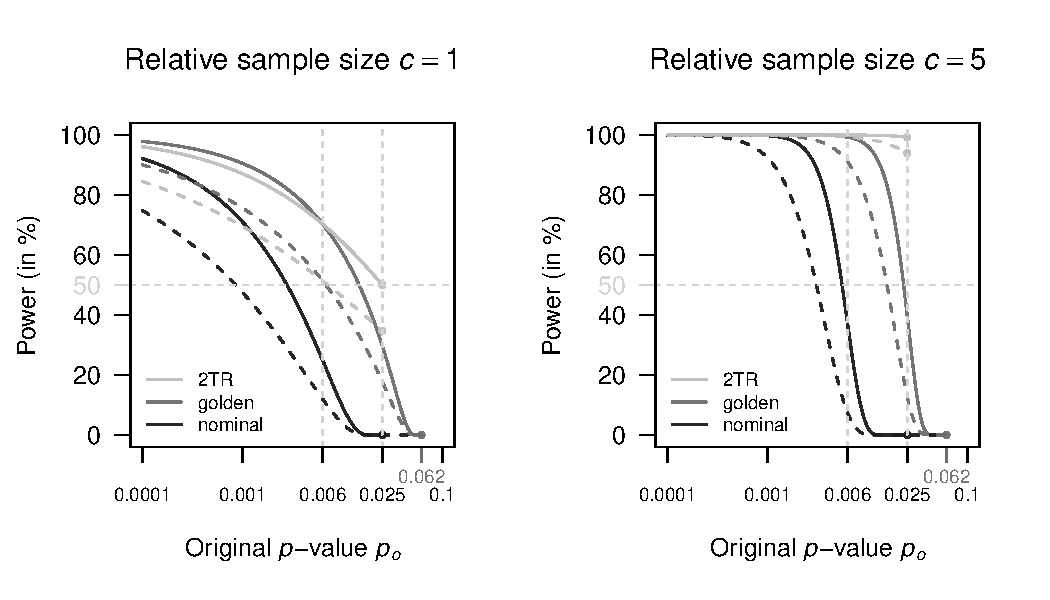
\includegraphics[width=\maxwidth]{images/paper1/fig3-1}

}

\end{knitrout}
\end{center}
\caption{Conditional power as a function of the {one-sided} $p$-value of the
  original study with relative sample size $c=1$ (left) and $c=5$ (right). Shown
  is conditional power assuming the unknown parameter is equal to the original
  effect estimate (solid) and conditional power based on 20\% shrinkage of the
  original effect estimate (dashed) for the two-trials rule (2TR) at level
  $\alpha = 0.025$ and for replication success at the corresponding golden and
  nominal level. Power values of exactly zero are omitted.}
\label{fig1:fig3}
\end{figure}

Figure~\ref{fig1:fig3} compares the power for replication success
\citep[see][Section 4 for details]{Held2020} at the golden and at the nominal
level with the power of the two-trials rule for relative sample size $c = 1$
(left) and $c = 5$ (right) as a function of the one-sided $p$-value $p_o$ from
the original study. Shown is the conditional power assuming the unknown
parameter $\theta$ is equal to the original effect estimate $\hat \theta_o$.
Then $\hat \theta_r \given \hat \theta_o \sim \Nor(\hat \theta_o, \kappa^2/n_r)$
and it follows that $d \given \hat \theta_o \sim \Nor(1, 1/(c z_o^2))$. The
conditional power for replication success can therefore be calculated as
\begin{equation}\label{eq1:condPower}
\P(d \geq \dmin \given \hat \theta_o) = \Phi\left[\sqrt{c} z_o (1-\dmin)\right],
\end{equation}
where $\dmin$ is given in \eqref{eq1:res}. Predictive power, which is conditional
power averaged over a $\Nor(\hat \theta_o, \sigma_o^2)$ distribution for the
effect size $\theta$, could also be calculated, then
\mbox{$d \given \hat \theta_o \sim \Nor(1, (1+1/c)/z_o^2)$}. Conditional and
predictive power of the two-trials rule also depend on $z_o$, $c$ and $\alpha$
and are given in \citet{Micheloud2020}.

The two-trials rule requires a significant original study and hence it is
impossible to power a replication study when $p_o > 0.025$. The same applies for
replication success at the nominal level, where the power is zero for any
$p_o > 0.025$, regardless of the replication sample size. This is different for
the golden level, where the conditional power of an original study with
$0.025 < p_o < 0.062$ is low, but not zero. However, if the original $p$-value
$p_o$ is slightly smaller than $0.025$, the two-trials rule has a larger power,
both for $c=1$ and $c=5$. But if the original $p$-value is sufficiently small
($p_o < 0.006$ for $c=1$), the power for replication success at the golden level
is larger than the power of the two-trials rule.


Compared to $c=1$, the conditional power for $c=5$ of both the two-trials rule
and the replication success approach at the golden level increases if
$p_o \leq \alpha$. A remarkable feature of the replication success approach at
the golden level is that conditional power can be pushed towards 100\% for large
enough $c$ if $p_o<\alpha$, but not otherwise. This can be seen from
\eqref{eq1:condPower} because $\dmin < 1$ for $p_o<\alpha$ and large enough
relative sample size $c$. On the other hand, for $p_o > \alpha$ conditional
power for replication success will tend to 0\% for increasing $c$ because
$\dmin>1$ for all $c$. Finally, for $p_o = \alpha$ the limit is 50\%. The same
property can be observed at the nominal level, however at the smaller threshold
$1-\Phi(z_\alpha \sqrt{\varphi})$ which is $0.006$ for $\alpha=0.025$. Only if
$p_o < 0.006$ will the conditional power for replication success attain 100\%
for $c \to \infty$. This further highlights the stringency of the nominal level.

The approach described so far takes the original study at face-value since it
assumes that $\hat \theta_o$ is equal to the unknown effect size $\theta$. In
practice, however, there are often good reasons to believe that original effect
estimates have a tendency to be inflated (\eg{} due to publication bias). One way
to address this issue is to base power calculations on a shrunken version of the
original effect estimate, where the amount of shrinkage is guided by domain
knowledge and a risk of bias assessment of the original study. For illustration,
Figure~\ref{fig1:fig3} also shows conditional power based on 20\% shrinkage of
the original effect estimate which reduces the conditional power for all
methods, especially for a relative sample size $c = 1$. Conditional power for
replication success at the golden level can now be pushed towards 100\% only for
$p_o < 0.018$, which can be derived by solving \eqref{eq1:alphaPrime} for
$\alpha$ with $\alpha'=0.025$ and $\dinfty=0.8$. To be able to push conditional
power based on 20\% shrinkage towards 100\% for all $p_o < 0.025$, equation
\eqref{eq1:alphaPrime} would have to be used directly to relax the level from
$\alpha=0.025$ to $\alpha'=0.033$.


\subsection{Overall Type I error rate}\label{sec1:T1E}
The two studies are assumed to be independent with Type I error rate fixed at
$\alpha$ for each of them, so the Type I error rate of the two-trials rule over
the entire project is simply $\alpha^2$ for any value of the relative effect
size $c$. In contrast, the Type I error rate of the proposed replication success
assessment {depends on} the relative sample size $c$.

For $c=1$, \citet[Section 3]{Held2020} showed that $z_S^2$ in
\eqref{eq1:extrinsic.p2} simplifies to half the harmonic mean of the squared test
statistics $z_o^2$ and $z_r^2$. The connection $z_S^2 = z_H^2/4$ to the harmonic
mean $\chi^2$-test statistic $z_H^2$ \citep{Held2020b}, which has a
$\chi^2(1)$-distribution under the null hypothesis, makes it straightforward to
compute the Type I error rate at level $\alpha_S$ for $c = 1$ as
\begin{eqnarray}\label{eq1:T1E}
\mbox{T1E} =   \left\{1-\Phi\left[2 \, \Phi^{-1}\left(1-\alpha_S \right)
 \right]\right\}/2.
\end{eqnarray}
For the golden level $\alpha_S =0.062$ at $\alpha = 0.025$, the Type I error
rate \eqref{eq1:T1E} is $0.0515$\%, slightly less than the Type I error rate
$\alpha^2=0.0625$\% of the two-trials rule. For comparison, the Type I error
rate at the nominal level $\alpha_S=0.025$ is $0.0022$\%, much smaller than
0.0625\%.


For $c \neq 1$, the Type I error rate can be calculated through numerical
integration:
\begin{equation}\label{eq1:T1E0}
  \mbox{T1E} = \int_{z_{\alpha_S}}^{\infty}
\P(z_r \geq \zrmin \given z_o, c, \alpha_S) \,
  \phi(z_o) \, dz_o,
\end{equation}
where $\phi(\cdot)$ denotes the standard normal density function. The first term
in the integral of \eqref{eq1:T1E0} is the probability of replication success at
level $\alpha_S$ conditional on a fixed original test statistic $z_o$ and a
relative sample size $c$. Now $z_r \sim \Nor(0,1)$ under the null hypothesis, so
this term simplifies to
$\P(z_r \geq \zrmin \given z_o, c, \alpha_S) = 1 - \Phi(\zrmin)$ where $\zrmin$
in \eqref{eq1:eq.z} depends on $z_o$, $c$, and $\alpha_S$.


\begin{figure}[!h]
\centering

\begin{knitrout}
\definecolor{shadecolor}{rgb}{0.969, 0.969, 0.969}\color{fgcolor}

{\centering 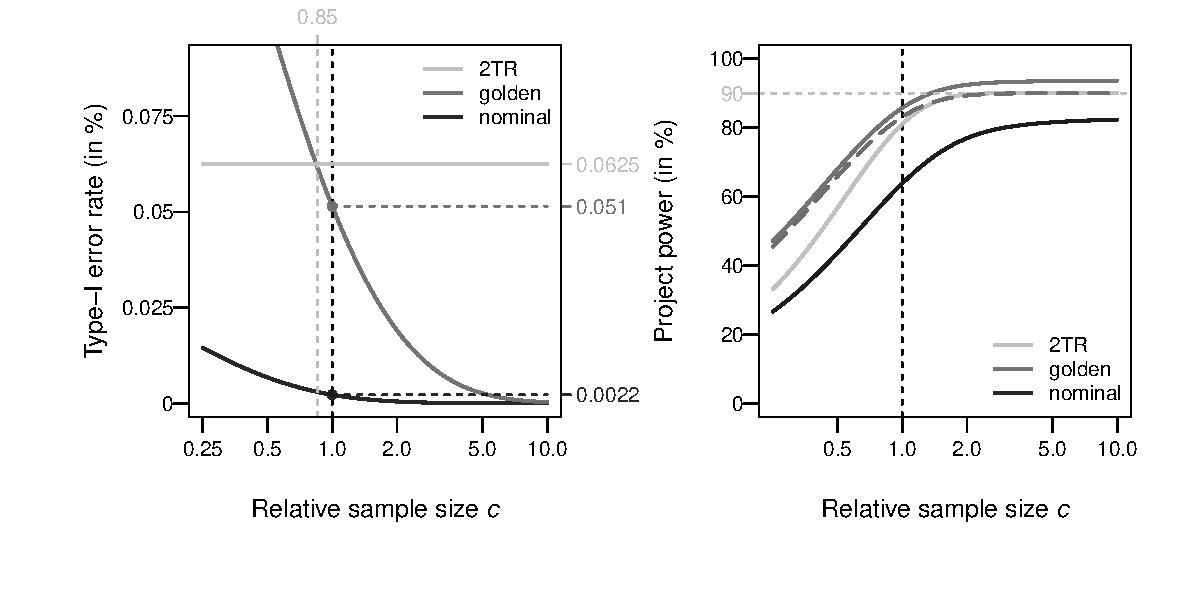
\includegraphics[width=\maxwidth]{images/paper1/fig4-1}

}

\end{knitrout}

\caption{Overall Type I error rate (left) and project power (right) for fixed
  relative sample size $c$. Results are given for replication success at the
  nominal and golden level and compared with the two-trials rule (2TR) at
  $\alpha = 0.025$. The dashed darkgrey line is the project power at the golden
  level based on significant original studies ($p_o \leq 0.025$). The power of
  the original study is 90\%.}
\label{fig1:fig4}
\end{figure}


The left plot in Figure \ref{fig1:fig4} displays the Type I error rate for
$\alpha=0.025$ as a function of the relative sample size $c$. It can be seen
that the Type I error of the replication success approach decreases with
increasing relative sample size $c$. This also follows from \eqref{eq1:T1E0}
where $\P(z_r \geq \zrmin \given z_o, c, \alpha_S) = 1 - \Phi(\zrmin)$ decreases
with increasing $c$, because $\zrmin$ increases with increasing $c$, see
equation \eqref{eq1:eq.z}.


The Type I error rate of the nominal level is always below the target
$0.0625$\%. Although the Type I error will eventually attain $\alpha^2$ in the
limit $c \downarrow 0$ \citep[Section 3.4]{Held2020}, the nominal level seems to
be too stringent for realistic values of $c$. The Type I error rate of the
golden level is smaller than $0.0625$\% for $c >0.85$. Appropriate Type I error
control is thus ensured even for replication studies where the sample size is
slightly smaller than in the original study.

\begin{figure}[!ht]
\begin{center}

\begin{knitrout}
\definecolor{shadecolor}{rgb}{0.969, 0.969, 0.969}\color{fgcolor}

{\centering 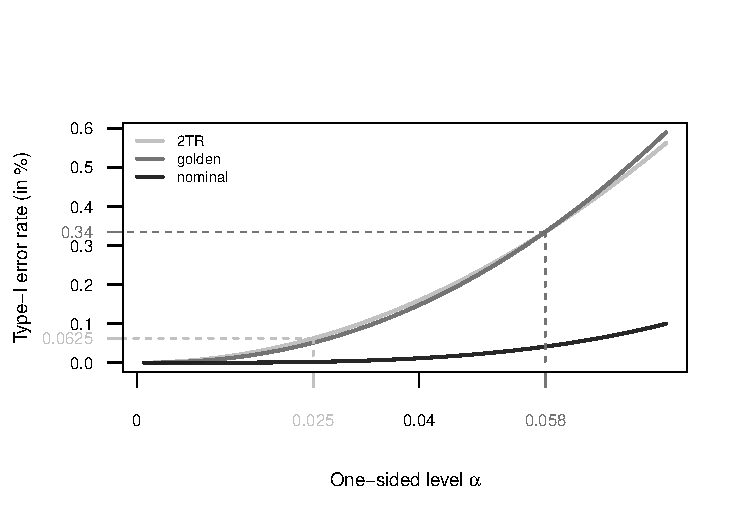
\includegraphics[width=\maxwidth]{images/paper1/fig5-1}

}


\end{knitrout}

\end{center}
\caption{Overall Type I error rate if the replication sample size equal to the
  original study ($c=1$). The two-trials rule (2TR) is compared to replication
  success at the golden and nominal level for different values of $\alpha$.}
\label{fig1:fig5}
\end{figure}

Figure \ref{fig1:fig5} compares for $c=1$ the Type I error rate \eqref{eq1:T1E} of
replication success at the golden and at the nominal level with the two-trials
rule for different values of $\alpha$. The Type I error rate of the two-trials
rule is $\alpha^2$ and the replication success approach at the nominal level
always has a much smaller Type I error rate than $\alpha^2$. At the golden level
the Type I error rate of the replication success approach is much closer to
$\alpha^2$, still slightly smaller if $\alpha < 0.058$. For $\alpha = 0.058$ the
Type I error rate is equal to the Type I error rate $0.058^2 = 0.34\%$ of the
two-trials rule and for $\alpha > 0.058$ the Type I error rate is slightly
larger than $\alpha^2$. The Type I error rate for replication success decreases
with increasing $c$, so as long as the replication sample size is not smaller
than the original sample size, Type I error control at $\alpha^2$ is guaranteed
at the golden level for any one-sided level $\alpha < 0.058$.

\subsection{Project power}\label{sec1:PP}
Under the alternative we have $z_o\sim \Nor(\mu, 1)$ with
$\mu = z_\alpha + z_\beta$ where $\alpha$ is the assumed significance level and
$1-\beta = \Phi(\mu - z_\alpha)$ is the power to detect the assumed effect
$\theta = \mu \sigma_o$ in the original study \citep[Section 3.3]{Matthews2006}.
In the following $\alpha=0.025$ and $\beta=0.1$ are used. The power of a
significant replication study with sample size $n_r = c n_o$ is
\begin{equation*}
\Phi(\theta/\sigma_r - z_\alpha) =
\Phi(\sqrt{c} \mu - z_\alpha),
\end{equation*}

so depends on $\mu$ and the relative sample size $c$. The project power of the
two-trials rule is therefore $(1-\beta) \, \Phi(\sqrt{c} \mu - z_\alpha)$ and
increases with increasing $c$.


The project power for replication success is computed as
\begin{equation*}
  \mbox{PP} = \int_{z_{\alpha_S}}^{\infty}
\P(z_r \geq \zrmin \given z_o, c, \alpha_S) \,
  \phi(z_o - \mu) \, dz_o
\end{equation*}
and shown in the right plot of Figure \ref{fig1:fig4} as a function of $c$. For
the golden level, the project power quickly increases to values above 90\%,
whereas the nominal level only reaches around 80\% project power. The project
power based on the two-trials rule is shown for comparison, which is always
smaller than for the golden level and converges to 90\% for large $c$.

The advantage in power stems partly from replication success still being
possible when the original $p$-value is larger than 0.025, but smaller than
0.062. If we assume that a replication study is only conducted if the original
study is significant (with $p_o \leq 0.025$), then the project power based on
the golden level (the dashed line in Figure \ref{fig1:fig4}) is slightly smaller
and for $c>1$ barely different than for the two-trials rule. More substantial
gains are still visible for $c < 1$. However, the restriction to original
studies with $p_o \leq 0.025$ may not reflect current practice in large-scale
replication projects. For example, 5 out of 143 replication studies considered
in Section \ref{sec1:application} do have original $p$-values between 0.025 and
0.062.


\section{Application}\label{sec1:application}
In this section, we illustrate the proposed methodology using data from four
replication projects. All four projects reported effect estimates that were
transformed to correlation coefficients ($r$). This scale allows for easy
comparison of effect estimates from studies that investigate different phenomena
and is bounded to the interval between minus one and one. Moreover, the Fisher
$z$-transformation $\hat{\theta} = \text{tanh}^{-1}(r)$ can be applied to the
correlation coefficients, resulting in the transformed estimates being
asymptotically normal with variance which is only a function of the study sample
size $n$, \ie{} $\Var(\hat{\theta}) = 1/(n - 3)$ \citep{Fisher1921}.



The first data set comprises the results from the \textit{Reproducibility
  Project: Psychology} \citep{Opensc2015}, whose aim was to replicate 100
studies, all of which were published in three major Psychology journals in 2008.
For our purpose only the 73 study pairs from the ``meta-analytic'' subset are
considered, since only for these studies the standard error of the Fisher
$z$-transformed effect estimates can be computed \citep{Johnson2016}. The second
data set comes from the \textit{Experimental Economics Replication Project}
\citep{Camerer2016} which attempted to replicate 18 experimental economics
studies published in two high impact economics journals between 2011 and 2015.
The third data stem from the \textit{Social Sciences Replication Project}
\citep{Camerer2018} where 21 replications of studies on the social sciences were
carried out, all of which were originally published in the journals
\textit{Nature} and \textit{Science} between 2010 and 2015. The last data set
originates from the \textit{Experimental Philosophy Replicability Project}
\citep{Cova2018} which involved 40 replications of studies from the emerging
field of experimental philosophy. Since only for 31 studies effective sample
size for original and replication study were available simultaneously, only
these pairs were included. For more information on the data sets see also
\citet{Pawel2020}.

\begin{table}[!ht]
    \centering
\caption{Results for each replication project:
Relative effect size $d$ (median with 25\% and 75\% quantiles on Fisher's $z$ scale), proportion of
successful replications with the two-trials rule (2TR) and the replication success (RS)
approach (at the golden level), and number of studies where the methods disagree.}
% \resizebox{\textwidth}{!} {
% latex table generated in R 4.0.5 by xtable 1.8-4 package
% Fri Nov 25 12:12:30 2022
\begin{tabular}{lcccc}
  \toprule
Project & relative effect size $d$ & 2TR (\%) & RS (\%) & discrepant \\
  \midrule
Psychology & 0.29 [0.03, 0.77] & 28.8 & 30.1 & 3/73 \\
  Experimental Economics & 0.67 [0.35, 0.92] & 55.6 & 55.6 & 0/18 \\
  Social Sciences & 0.52 [0.13, 0.65] & 61.9 & 52.4 & 2/21 \\
  Experimental Philosophy & 0.86 [0.47, 1.12] & 74.2 & 71.0 & 1/31 \\
   \bottomrule
\end{tabular}

% }
\label{tab:marginalres}
\end{table}

Table~\ref{tab:marginalres} presents overall results for each of the replication
projects. While the median relative effect size is below one for all of the four
projects, there are still large differences. For example, the median relative
effect size is only $0.29$ in the Psychology project, whereas it is $0.86$ in
the Philosophy project. The degree of shrinkage is also reflected in the success
rates (according to the two-trials rule and the replication success approach at
the golden level), which are around 30\% for the former and more than 70\% for
the latter. The proportion of successful replications is similar for the
two-trials rule and the replication success approach. In the Experimental
Economics project the methods perfectly agree, while in the other three projects
the methods disagree for a few studies.

\begin{figure}[!h]
\centering
\begin{knitrout}
\definecolor{shadecolor}{rgb}{0.969, 0.969, 0.969}\color{fgcolor}

{\centering 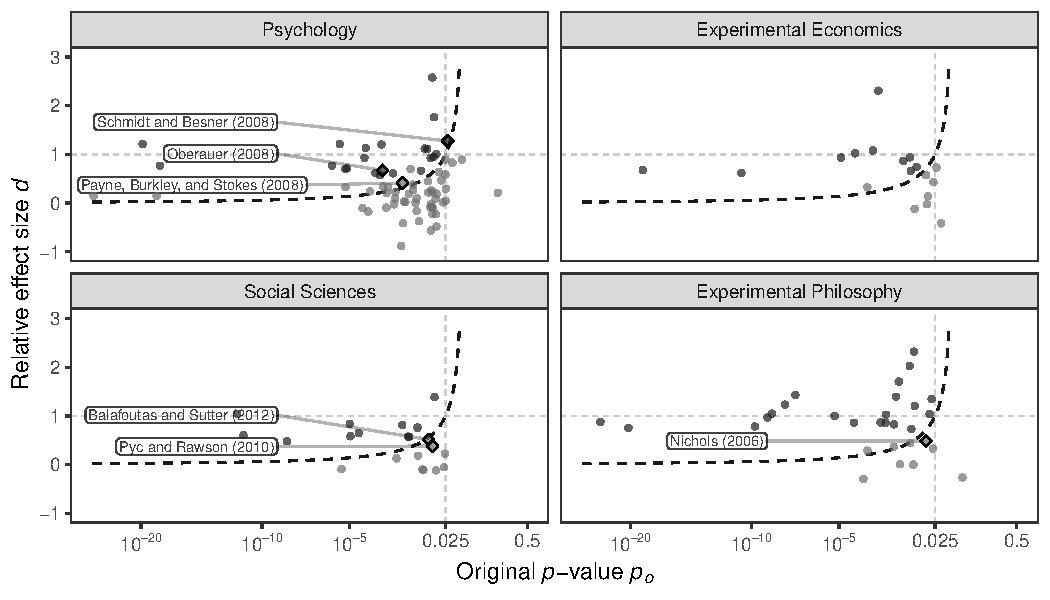
\includegraphics[width=\maxwidth]{images/paper1/fig6-1}

}


\end{knitrout}
\caption{Relative effect size $d$ versus original $p$-value $p_o$. Black
  indicates that replication success was achieved at the golden level while grey
  indicates that it was not. The diamonds mark studies where the replication
  success approach (at the golden level) and the two-trials rule disagree. The
  dashed black line indicates the limiting relative effect size at the golden
  level with $\alpha = 0.025$. }
\label{fig1:fig6}
\end{figure}


Figure~\ref{fig1:fig6} displays the relative effect size $d$ versus the original
$p$-value $p_o$ for each study pair and stratified by project. Note that one
study pair from the Philosophy project is not shown due to extremely small
original $p$-value and another study pair from the Psychology project is not
shown due to a very large relative effect size. We can see that for most of the
study pairs, the replication success approach and the two-trials rule lead to
the same conclusion, only six replications show conflicting results. They are
highlighted with diamonds in Figure~\ref{fig1:fig6} and their characteristics are
summarised in Table~\ref{tbl:discrep}.
\begin{table}[!ht]
    \centering
  \caption{Characteristics of studies for which the replication success approach
    (at the golden level) and the two-trials rule disagree (at one-sided
    $\alpha = 0.025$). Shown are relative sample size $c$, relative effect size
    $d$, original, replication and recalibrated sceptical $p$-value $p_o$, $p_r$
    and $\tilde{p}_S$.}
  \label{tbl:discrep}
\resizebox{\textwidth}{!} {
% latex table generated in R 4.0.5 by xtable 1.8-4 package
% Fri Nov 25 12:12:30 2022
\begin{tabular}{lllllll}
  \toprule
Study & Project & $c$ & $d$ & $p_o$ & $p_r$ & $\tilde{p}_S$ \\
  \midrule
\citet{Schmidt2008} & Psychology & 2.58 & 1.28 & \textbf{0.028} & \textcolor{black}{< 0.0001} & \textcolor{black}{0.024} \\
  \citet{Oberauer2008} & Psychology & 0.60 & 0.67 & \textcolor{black}{0.0003} & \textbf{0.035} & \textcolor{black}{0.017} \\
  \citet{Payne2008} & Psychology & 2.65 & 0.41 & \textcolor{black}{0.001} & \textcolor{black}{0.023} & \textbf{0.031} \\
  \citet{Balafoutas2012} & Social Sciences & 3.48 & 0.52 & \textcolor{black}{0.009} & \textcolor{black}{0.011} & \textbf{0.04} \\
  \citet{Pyc2010} & Social Sciences & 9.18 & 0.38 & \textcolor{black}{0.011} & \textcolor{black}{0.004} & \textbf{0.061} \\
  \citet{Nichols2006} & Experimental Philosophy & 9.40 & 0.49 & \textcolor{black}{0.015} & \textcolor{black}{0.0006} & \textbf{0.049} \\
   \bottomrule
\end{tabular}%
}
\end{table}
Two studies from the Psychology project show replication success but fail the
two-trials rule. These studies show $p$-values that are slightly above the
significance threshold in either original or replication study, but do not
exhibit much shrinkage; in the replication of \citet{Oberauer2008}, the
replication $p$-value was $p_r = 0.035$, a little too large to pass the
two-trials rule. However, as the replication effect estimate shrunk only about
$30$\% compared to the original one, replication success is still achieved.
Conversely, the original $p$-value $p_o = 0.028$ in \citet{Schmidt2008} was just
above the significance level, yet the replication led to a highly significant
result $p_r < 0.0001$ with the effect estimate being even $30$\% larger than the
original counterpart, which therefore also resulted in replication success.

The remaining conflicting studies do not show replication success despite
passing the two-trials rule. In all cases, there is substantial shrinkage of the
replication effect estimate compared to the original one. For instance, in the
replication study of \citet{Pyc2010}, the estimate shrunk by $62$\% and the
replication $p$-value was only significant because the sample size was increased
by a factor of $c = 9.2$.



This analysis was based on the default choice $\dinfty=1$ at $\alpha=0.025$ for
the golden level as described in Section \ref{sec1:goldenthresh}. We may also
choose a different value for the limiting relative effect size $\dinfty$ at
$\alpha=0.025$ which then corresponds to $\dinfty=1$ at a different level
$\alpha'$ as given in \eqref{eq1:alphaPrime}. Figure \ref{fig1:fig7} compares the
proportion of successful replications with the replication success approach for
$\dinfty \in (0.5, 1.1)$ with the two-trials rule at the
corresponding levels
$\alpha' \in (0.06, 0.022)$ for
all four replication projects. We can see that the two proportions agree fairly
well for all values of $\alpha'$ considered. The number of discrepant studies in
each project varies between 0 and 3. Only in the Psychology project there are
some studies which are successful with the replication success approach but not
the two-trials rule and some studies successful with the two-trials rule but not
the replication success approach. The proportion of studies where both methods
are successful (also shown in Figure \ref{fig1:fig7}) is then smaller than the
proportion of successful replications with either one of the two methods. The
three discrepant studies from the Psychology project listed in the top three
rows of Table~\ref{tbl:discrep} are an example of this particular feature.

\begin{figure}[!htb]
\begin{knitrout}
\definecolor{shadecolor}{rgb}{0.969, 0.969, 0.969}\color{fgcolor}

{\centering 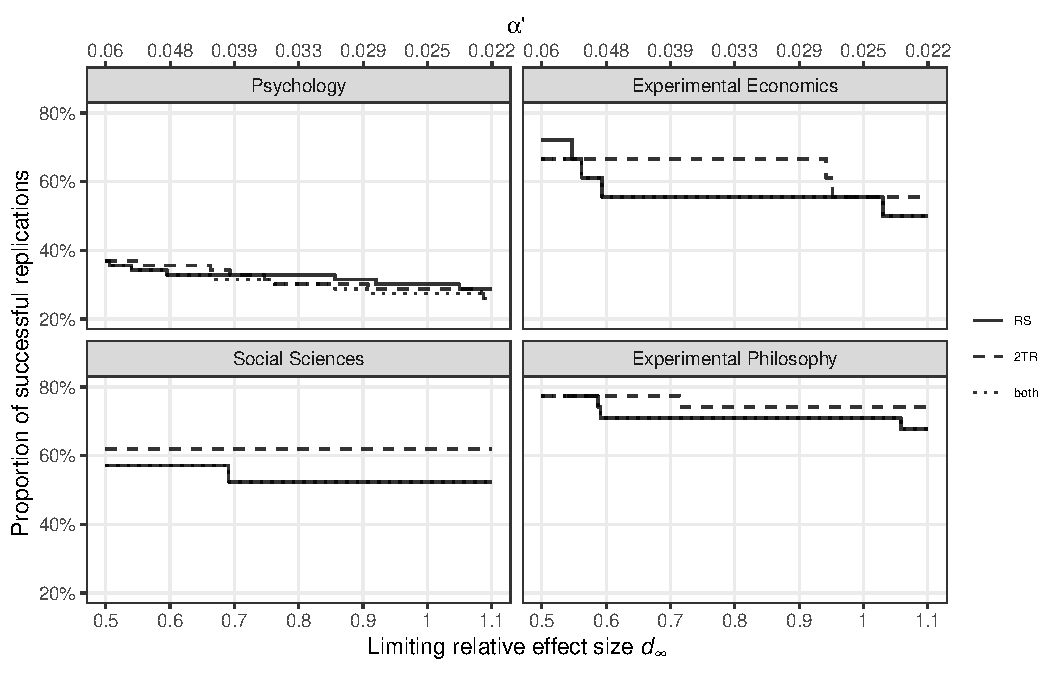
\includegraphics[width=\maxwidth]{images/paper1/fig7-1}

}

\end{knitrout}
\caption{Proportion of successful replications as a function of the limiting
  relative effect size $\dinfty$ at $\alpha = 0.025$. The upper axis gives the
  equivalent level $\alpha'$ where the corresponding limiting relative effect
  size is 1. The replication success (RS) approach is compared with the
  two-trials rule (2TR).}
\label{fig1:fig7}
\end{figure}



\section{Discussion}\label{sec1:discussion}
In this paper, we have expanded on the replication success approach introduced
in \citet{Held2020} and demonstrated its advantages over alternative methods
such as the two-trials rule. In particular, the method provides an attractive
compromise between hypothesis testing and estimation,
as it penalizes
shrinkage of the replication effect estimate compared to the original one,
while ensuring that both are statistically significant to some extent.
%% For instance, the method will indicate only a low degree of replication success when
%% the replication study shows a much smaller but statistically significant
%% effect estimate, whereas it can still indicate some degree of
%% success when either original or replication $p$-value are slightly above the
%% significance level. %% , provided their effect estimates are compatible.

We further refined the method by proposing the golden level, a new threshold for
replication success. It guarantees that borderline significant original studies
can only be replicated successfully if the replication effect estimate is larger
than the original one. Compared to the two-trials rule, the golden level offers
uniform gains in project power and controls the Type I error rate at any
one-sided level $\alpha < 0.058$ if the replication sample size
is not smaller than the original one. Empirical evaluation of data from four
replication projects highlights that in most cases the methods are in agreement,
however, for the study pairs where the approaches disagree, the replication
success approach seems to lead to more sensible conclusions. The good
performance has been recently confirmed by a comparison of different replication
success metrics through a simulation study in the presence of publication bias
\citep{Muradchanian2021}.

Despite a lack of agreement as to which statistical method should be used to
evaluate replication studies, conclusions based on different methods usually
agree. Nevertheless, in some cases, classical methods such as the two-trials
rule may produce anomalies. We argue that the replication success approach
improves upon existing methods leading to more appropriate inferences and
decisions that better reflect the available evidence. However, in extreme cases
the performance of the sceptical $p$-value may be considered as strange or even
counterintuitive. Specifically, if the original study was only borderline
significant, a highly significant replication study can only lead to success if
the replication effect estimate is larger than the original one. To understand
this behaviour it is important to realize that the proposed approach does not
synthesize the evidence from the two studies (like a standard meta-analysis).
The sceptical $p$-value is designed to confirm claims of new discoveries through
replication, but will remain ``stubborn'' \citep{Ly2020} if the original study
was not particularly convincing, even if the replication study provides
overwhelming evidence for an effect. It will lead to a different result if the
order of studies was reversed, as long as original and replication study do not
have the same sample size ($c \neq 1$). The related harmonic mean $\chi^2$-test
\citep{Held2020b} for evidence synthesis of two or more studies also requires
each study to be convincing on its own to a certain degree, but treats them as
exchangeable.

With this paper we further advanced the reverse-Bayes methodology for the
analysis and design of replication studies, yet certain limitations and
opportunities for future research remain: First, assuming normality of the
effect estimates may be questionable, especially for small sample sizes, and
more robust distributional assumptions could be considered. Second, in some
types of analyses (\eg{} regression or ANOVA) the effect estimate is a vector and
the approach would need suitable adaptations. Third, there is a recent trend to
not only conduct one but several replications for one original study
\citep[\eg{}][]{Klein2014, Ebersole2016, Klein2018}. Also for this situation, the
method would need to be adapted, \eg{} the replication estimates could be first
synthesized and an analysis of replication success could be performed
subsequently.


Throughout the paper we have assumed that the relative sample size is fixed in
advance. In practice the sample size of the replication study is often chosen
based on the result of the original study \citep{Anderson2017}. Power
calculations as shown in Figure \ref{fig1:fig3} can then be inverted to determine
the appropriate sample size of the replication study. We can also invert
equation \eqref{eq1:res} to obtain the required replication sample size based on
the specification of the minimum relative effect size $\dmin$ to achieve
replication success. This novel way of calculating the sample size requires the
specification of the minimum relative effect size which can still be considered
as acceptable. Sample size calculations based on the two-trials rule can also be
formulated in terms of the minimum relative effect size by inverting equation
\eqref{eq1:dSig}. We will report on a detailed comparison of the different
approaches in future work.



\section*{Data and Software}
Code and data to reproduce our analyses are available at
\url{https://github.com/SamCH93/RSgolden/}. A snapshot of the Git repository at
the time of writing is archived at \url{https://doi.org/10.5281/zenodo.XXXXXX}.
The data which was used is available in the R package
\texttt{ReplicationSuccess} (available on CRAN). Further information can be
found on the corresponding help page (with the command \texttt{?RProjects}).

\section*{Acknowledgments}
Support by the Swiss National Science Foundation (Project \#~189295) is
gratefully acknowledged. We acknowledge helpful and constructive comments by the
editor and a referee on an earlier version of this article.


\bibliographystyle{apalikedoiurl}
\bibliography{bibliography}
